\scanpage{12}
de \inserted{\unsure{hypo}} platitude sur les $Q^0[M^\bullet]$ et les $\mathcal H^i(Q^0(M^\bullet))$, \deleted{\unsure{qui en sont}} soit (plus économiques, sans doute, vu que l'on ne peut guère avoir de platitude sur $\underline O_X$ de $Q^0[M^\bullet]$ sans celle de $X^{\widehat{[1]}}\unsure{-|\longrightarrow}X^0$\unsure{]|)} une hypothèse de ``\uline{platitude infinitésimale de} $X/S$'' i.e. \inserted{une hypo. de \deleted{\unsure{pro}} platitude sur} $X^{\widehat{[1]}}\unsure{-|\longrightarrow}X$ --- p.ex. $X/S$ plat
\[
\cdots\quad[\text{critères : dégager}].
\]
Alors
\margin{\figure{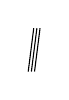
\begin{tikzpicture}[x=1cm,y=1cm]
\draw (0,0)--(.07,.55);\draw (.04,0)--(.11,.55);\draw (.08,0)--(.15,.55);
\end{tikzpicture}}}
\deleted{\unsure{(a)}} $1^\circ)$ Les $V^i=\mathcal H^i(\ell Q^0[M])$ sont de façon naturelle des $\underline O_X$-Modules (par la \inserted{$\underline O_X$-}structure gauche) \uline{stratifiés}.

$2^\circ)$ Dans le bicomplexe $\ell Q^*[M^\bullet]$, prenant les \inserted{faisceaux de} cohomologie suivant l'op. diff. provenant de $M^\bullet$ nous donne précisément les \deleted{\unsure{$Q$}} complexes $C^\bullet(V^i)$ attachés aux \deleted{connexions}\inserted{stratifications} des $V^i$.

$3^\circ)$ Par suite, on trouve une suite spectrale
\margin{11}
